\documentclass[a4paper,10pt]{article}
\usepackage[utf8]{inputenc}
\usepackage{graphicx}

%opening
\title{MSc Dissertation}
\author{Jose Rodriguez}

\begin{document}

\maketitle

\begin{abstract}

\end{abstract}

\section{Methodology}

This section will discuss the method used, which overall consits in three sequential steps, evaluating the model on the training set of the GSM8K to filter the questions where the models parameters are less aligned to answer, then iteritevely generating new answers over this section of the dataset, preparing sets of data with the appropiate format to be used for training, and using different methods for training the model. The resulting models from the training stage will be evaluated on the test set of the GMM8K using the same process as the filtering stage of the training set.

%\begin{figure}[h]
%\centering
%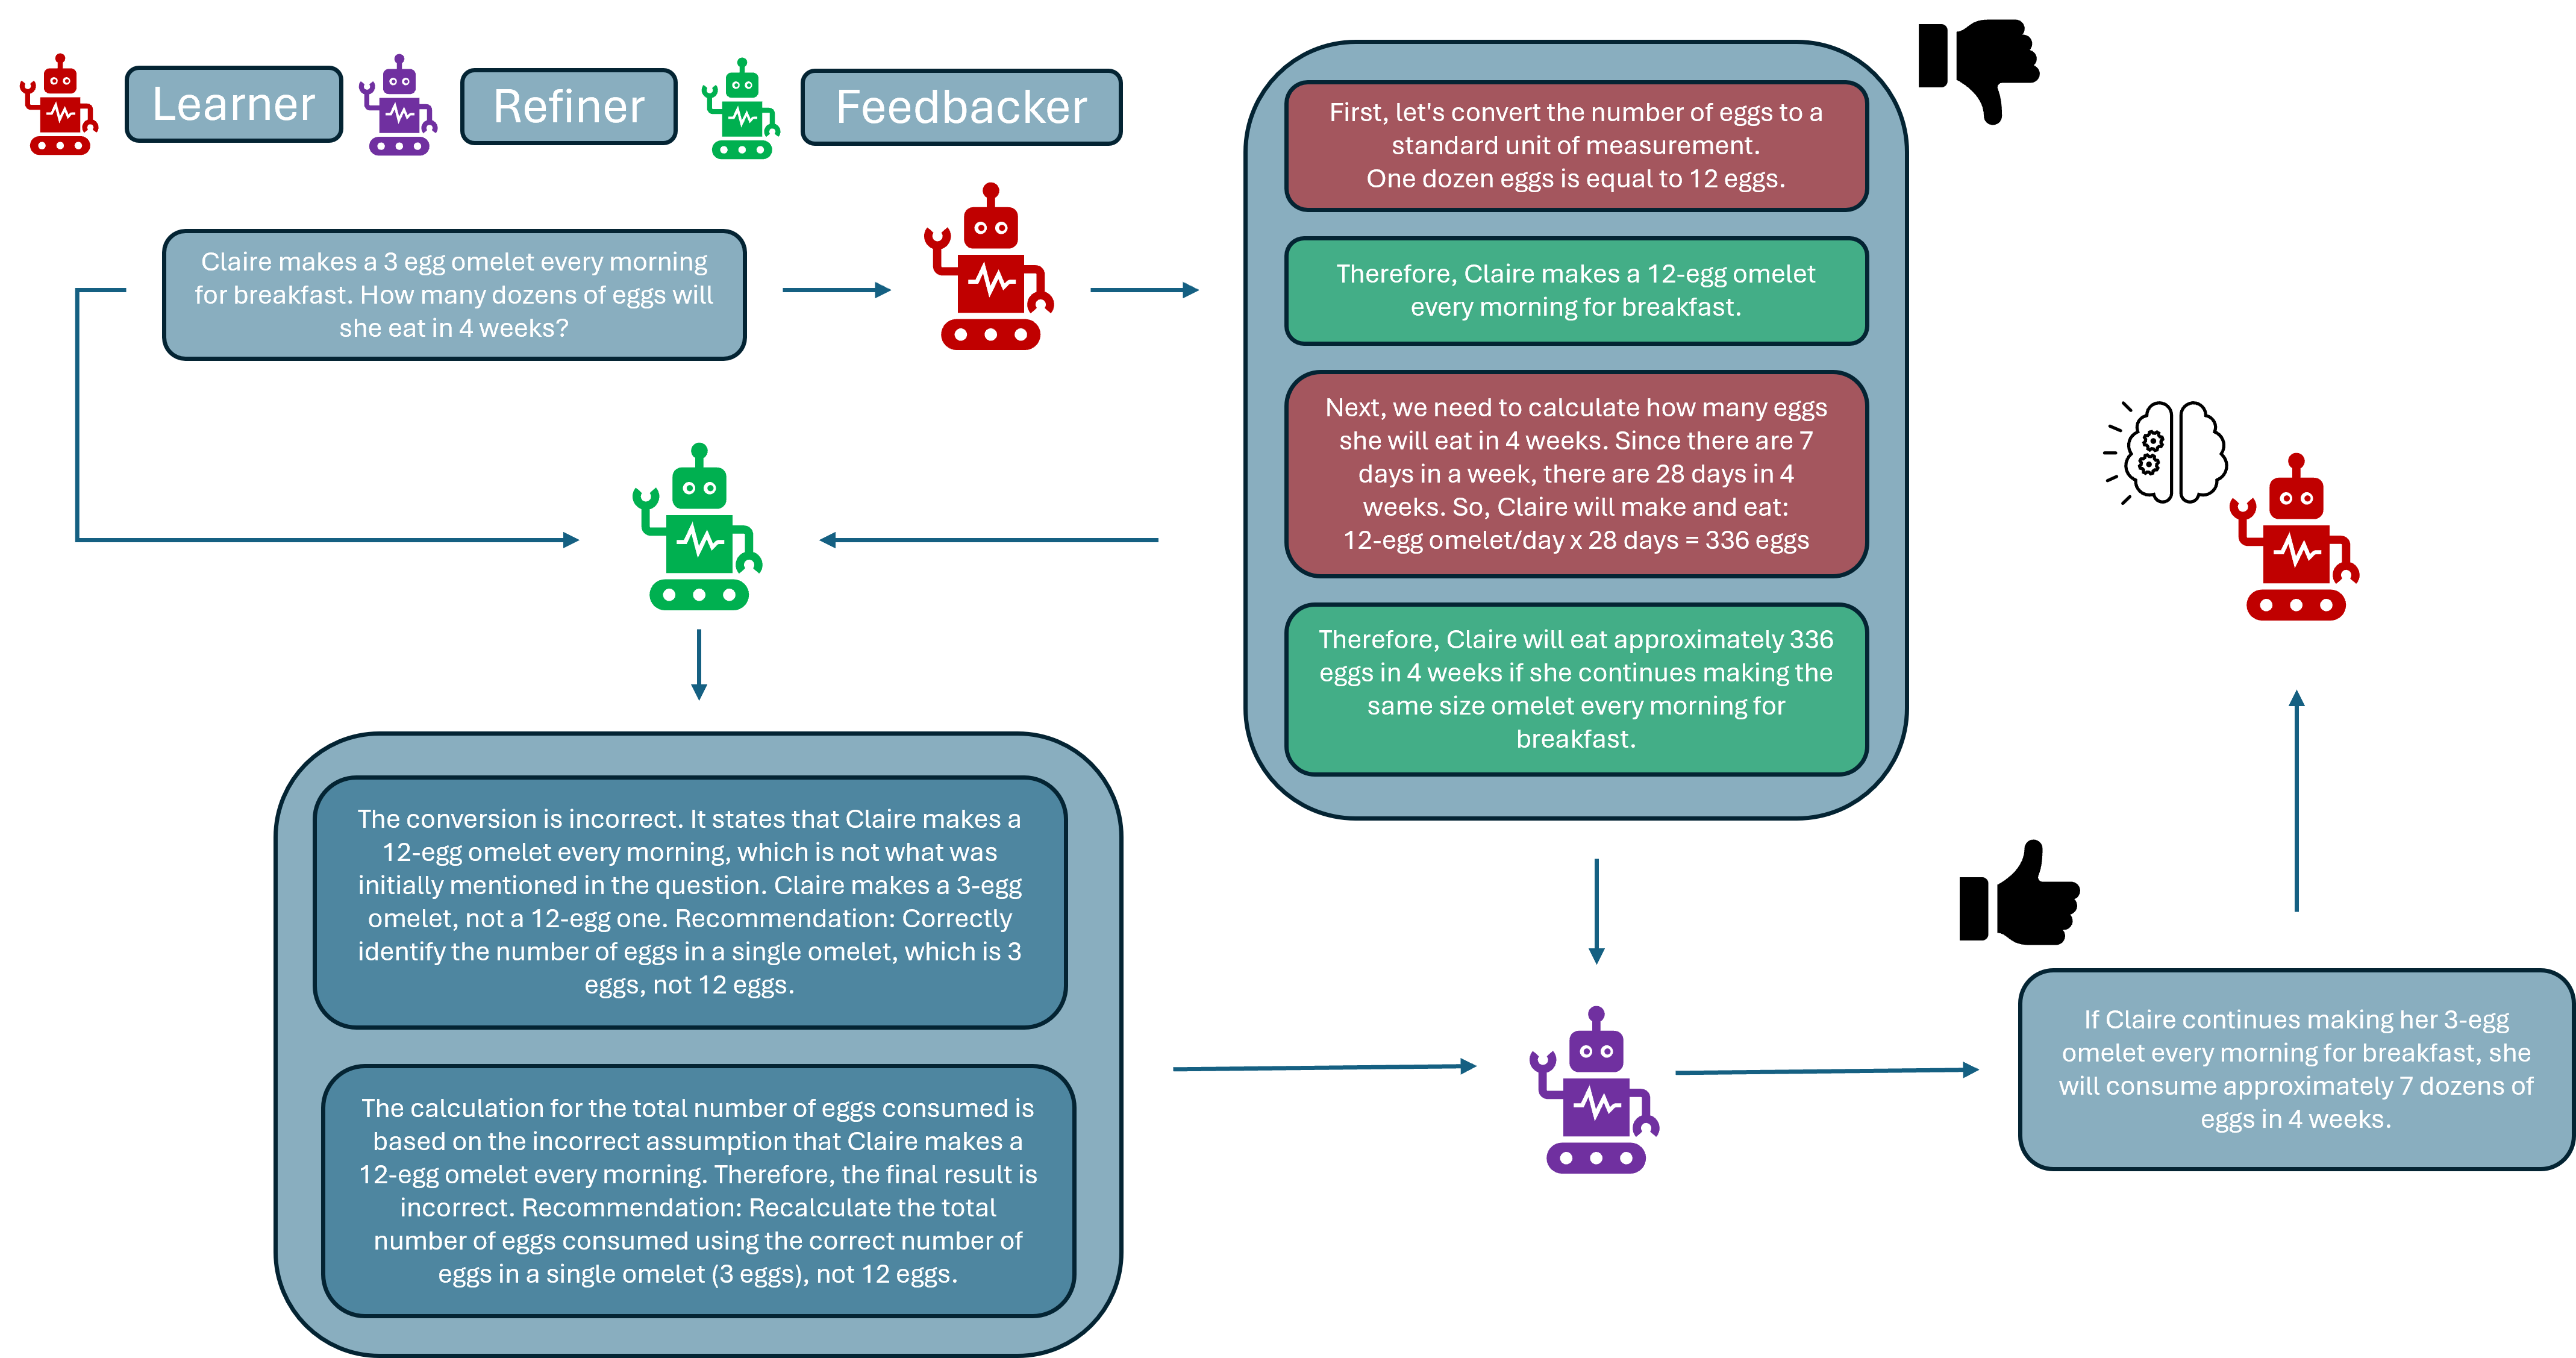
\includegraphics[scale=0.3]{figures/method_sample}
%\caption{Overview of the mechanism}
%\end{figure}


\subsection{Train Set Filtering}
We identify the set of hardest questions by evaluating the learner model on the train set, which in this case is on the task of question answering of the GSM8K. For $N$ responses we extract the last number of the sequence which is matched again the expected numerical response. We consider this set as the hardest questions for the model in the dataset, which would be expressed as follow. $ hard_q =  N - easy_q $ with $easy_q$ represented as the questions that the model generated a correct answer.
In our case using LLAMA3-8B-IT with zero-shot CoT resulted on $ 2085 = 7473 - 5388 $ We proceed to iterate over this set, as the feedback to be provided assumes that the answer is incorrect, also as we conjecture that the parameters to the models are suficiently aligned to answer the easier questions.
\subsection{Data Generation}
The incorrect responses are repaired by a process of iteritevely exchange generation between two models, one for feedback and another one for refinement, which in practice is the same model with different prompting. This procedure is repeated over all the unsolved questions until a stop criteria is met. Similarly to ILF we also generate the new feedbacks and responses over the list of previous tries in order to ensure that the model is trying different solutions.
\paragraph{Feedback Generation}
Each question has a set of feedback generated, which will be equal to the size of amount of iterations. Generation is done in chat format, firstly the model is instructed that the user will ask for feedback, and the answer is always wrong and that feedback must  be provided atomically identifying the incorrect steps in the answer. The role of the user contains the question that was attempted to answer, and the answer initially generated by the model, then feedback is generated as an assistant message. This is repeated through all the incorrect responses, iteritevely, replacing the initially wrong answer by the last refinement where the provided feedback was applied.
\paragraph{Refinement Generation}
Similar to feedback generation, each question will have a list of refinements which size will be equal of the amount of iterations. The model is instructed that given a question from the user, and a incorrect answer from itself, the user will provide feedback and the model must apply the feedback and generate an improved version. Generation is done through a chat template and the messages from the user is the feedback generated in the previous step. The generation starts with the initially incorrect answer generated in the filtering step from the training set and the feedback generated for that answer by the feedback model, the process is then repeated iteritevely, adding the new refinements  attempts and the feedback for it to the chat until a correct solution is found.
\paragraph{Stopping Criteria}
The process of generating feedback and refinement for reach question will eaither stop because all question have a refinement with the correct answer, which is correctness is provided by the verifier, or because a max number of passes previously specified has been reached. Another edge case in which the process will end, which in our case was the main reason, is that the resources (like memory gpu) have been exhausted.
\paragraph{Verifier}
The verifier changes depending on the nature of the task, the main purpose is simply to provide the correctness of an answer, which in our case of QA, was simply a boolean if the answer was correct or not. This was computed by extracting the last numerical expresion of the string, and compare it to the expected number for that answer. This comparison can be strictly or flexibly made, the former must match a prefix and the exact number, the latter just needs to match the number, and this will match even if it has some symbol preceeding (eg. a dollar sign). We evaluate our mechanism mainly sing the latter. The same verifier is for the stop criteria and for the performance evaluation of the model, which comes from lm-eval-harness


\subsection{Data Preparation}
Initially we build a dataset only using the generated correct refinements, which then will be prepared for training in with QA format for the model to be trained on. Later we try different combinations of all the generated data and gold labels.
\paragraph{Formatting}
Fundamentally, we go through all the hard question that have been solved through the feedback and refinement loop, and the corresponding generated correct answer and wrap them as a multi-turn chat, with the question being a prompt from the user with zero-shot CoT and the expected answer to be generated as response from the assistant. Empirically we found that sanitizing the refinement leads to better results, in this case we removed the first sentence for the target answer to be generated, as it had conversational dialogue due to the context it was being generated, and replace it with the most common sentence generated by the model in the set of correct answers generated through the filtering stage. 
\paragraph{Experimental Setup}
In principle our method is a data curation mechanism, as we aim to find a set of sequences, minimal in size that maximizes accuracy on the GSM8K, different combinations of data used in the training have been reported and discussed through this work. All of the following sets are structured in QA format, the sentence of the question remains unaltered from the original dataset. What changes with the different combinations is the set of which questions and the answers, which may be generated by the model (sanitized or unsanitized) and the gold labels from the GSM8K. 

The initially proposed set from our method is \textbf{hard-q solved} which answers are generated through the refinement process on the filtered $hard_q$ and amounts to ~940 instances after 7 passes. \textbf{Tsolved} are all the answers generated by the model $Tsolved = hard_q + easy_q$.  \textbf{hardq sovled with gold} fills the questions that the model was not able to answer in the refinement process with the gold labels of the dataset, the size of the set being equal to the size of $hard_q$.\textbf{all solved with gold} would be expressed as $N = Tsolved + gold$ which equals to $hard_q$ solved with gold plus $easy_q$. \textbf{hardq full gold} refers to the set which all the hard question ideintified in the filtering ($hard_q$) will be paired not with the answers generated by the model but instead with the gold labels, this set will be equal in size to $hard_q$. \textbf{full gold} of size $N$ is the entirety of the questions of the GSM8K paired with it correspondig gold labels. \textbf{unsolved with gold} are the questions that could not be solved neither in the initial filtering stage or in the refinment process, paired with the corresponding gold labels, the size of the set is computed as $unsolved_q = hard_q - (hard_q solved)$ resulting in 1140. The configuration that contains gold labels, in some experiments will be refered with \textbf{prefix} and it means that the gold label is preceed with the most common first sentence geenrated by the model. When using the term \textbf{sanitized} with the generated refinments, we mean that the first sentence of the sequence is replaced also with the most common first sentence generated by the model in the initial filtering of the training set. Aditionally, refinments that directly contain the answer and do not contain the steps that lead to that answer were removed during this process, which in our experiments amounted to 7 instances. \textbf{NOTE remember now to talk about filthy and double sanitized}
\subsection{Training}
Using all the data collected during the data preparation stage, we template each row as a QA task in a chat setting as a multiturn conversation, the question being an instruction from the user asking for an answer with zeroshot prompting, and the target to predict the response from the assistant. All the experiments regarding training in this work have been done on the same model as generation, which in this cas is LLAMA38B-IT. We test the performance of the data with two methods, Supervised Fine-Tunning (SFT) and Direct Preference Optimization (DPO). We took into consideration memory optimization for the training process due to hardware constrains, for this we used Low-Rank-Adaptations (LORA) and 4-bit quantization.
\paragraph {Memory Optimization}
Due to memory constrains we took into configuration two simple methods that allowed us to maximally update the models parameters relative to the loss function, that would fit into a single A100 45GB GPU. The LORA is done by adding a new smaller set of parameters that will be optimized, while the original parameters of the model remain freezed. This smaller set of parameters is updated to optimize the loss function. Futher optimization was required to fit the model in memory in a way that the low rank adaptation matrixes could be updated, for this we use a 4-bit quantization of the model parameters, which transforms the original 32-bit floating point parameters to 4-bit floating point numbers, without signifincatly reducing the accuracy of the model. 
\paragraph{Supervised Fine-Tunning (SFT)}
When the data is already formatted and tokenized, we firstly experimented by updating the parameters based on the loss of the whole sentence, including the prompt which contains the instruction of the user, empirically we found that computing the loss only on the expected sequence to be generated which is the response from the assistant with the answer yields greater results. All of the experiments with SFT showed in this work (unless stated otherwise) were ran on 500 steps, with the same learning rate LORA configuration and 4-bit quantization.
\paragraph{Direct Preference Optimization (DPO)}
We explored how our method would perfomr with DPO by creating a dataset of choosen and reject generations, where the choosen are the correct refinements and the rejected are the initially incorrect answer generated. This experiments ran over 5000 steps, with the same LORA configuration and quantization as SFT. We tested DPO directly from the choosen and rejected pairs dataset, also by running DPO in the resulting model from SFT, and also tried with a different a loss from \textbf{CITE RPO LOSS} which reported promising results. Few experiments were done on this method due to the low performance on this dataset.

\section{Dataset}
We used the same dataset for all the experiments accross this work. The GSM8K is an industry standard metric to evaluate LLMs promblem solving ability, which would allow us to do a fair comparison against the current state-of-the-art methods. To do this, it frames math world problems as a question answering task, which has been a long standing area of research in the NLP community. 

\paragraph{Question and Answering Generation (QA)}
In the context of this work we refer to QA as a task, where an LLM is prompted with question, and is expected to generate an answer. For the model to be trained with this task, it receives  a set of QA pairs, and the model parameters will be updated to optimize the loss between the generated answer and the expected answer. The trained model will then be evaluated on this task by introducint a sequence with the question and expecting the model to generate an answer, which validity will be verified differently depending on the task, in our case we discritly evaluate, it would be either correct or wrong and we use that information to compute the models accuracy.

\paragraph{Math World problems (MWP)}
A math word problem is a mathematical exercise where a significant part of the background information is presented in texts as natural language, rather than in mathematical notation (Part I ``Solving Arithmetic Mathematical Word Problems: A Review and Recent Advancements'' Chandra et al. (2019)). These problems are part of the basic elementary school curriculum, starting with basic operations(addition, subtraction, multiplication, division), and as the students advance problems contain higher levels of complexity (e.g., rate, probability, permutation, combination). Solving this problem requires linguistic and reasoning comprehension, thus the study of how children solve them has been a challenging area of research in cognitive science and education psychology (Part I ``Solving Arithmetic Mathematical Word Problems: A Review and Recent Advancements'' Chandra et al. (2019))). As solving them requires linguistic abilities and reasoning along with knowledge of arithmetic operations, researchers on AI and NLP have studied this as a task of building a system capable of replicating the cognitive process of solving these problems. 

\paragraph{Grade School Math 8k (GSM8K)}
Introduced by [cite], a dataset on the task of QA with 7.47k on the train and 1.32k on the test split. Each question is a MWP and the answer contain two pieces of information, an integer which is the target value and value a \textbf{gold} answer written by a humman, it contains the steps that lead to the integer, with relevant algebraic operations and their result. The steps in the gold answer are similary structured, and separeted by new lines, and at the end clearly state the precise integer which steps led to, this is what will be used as a label and will be used to determine if the answer is correct or not, independently of the steps. A metric on how ``hard'' a question is would be the amount of steps in the gold lead to the integer value. This dataset was a suitable candidate to test our hypothesis thanks to writing style that elicit in the model, which we conjecture that is esier to iterate as it can be approached atomically by the model by providing feedback to each step that led to the answer. Each problem is relatively unique, preventing the model from exploiting common patterns in the solving of the problems therefore allowing us to conduct better research on how the model can generalize its reasoning to solve the problems.

%\begin{figure}[h]
%\centering
%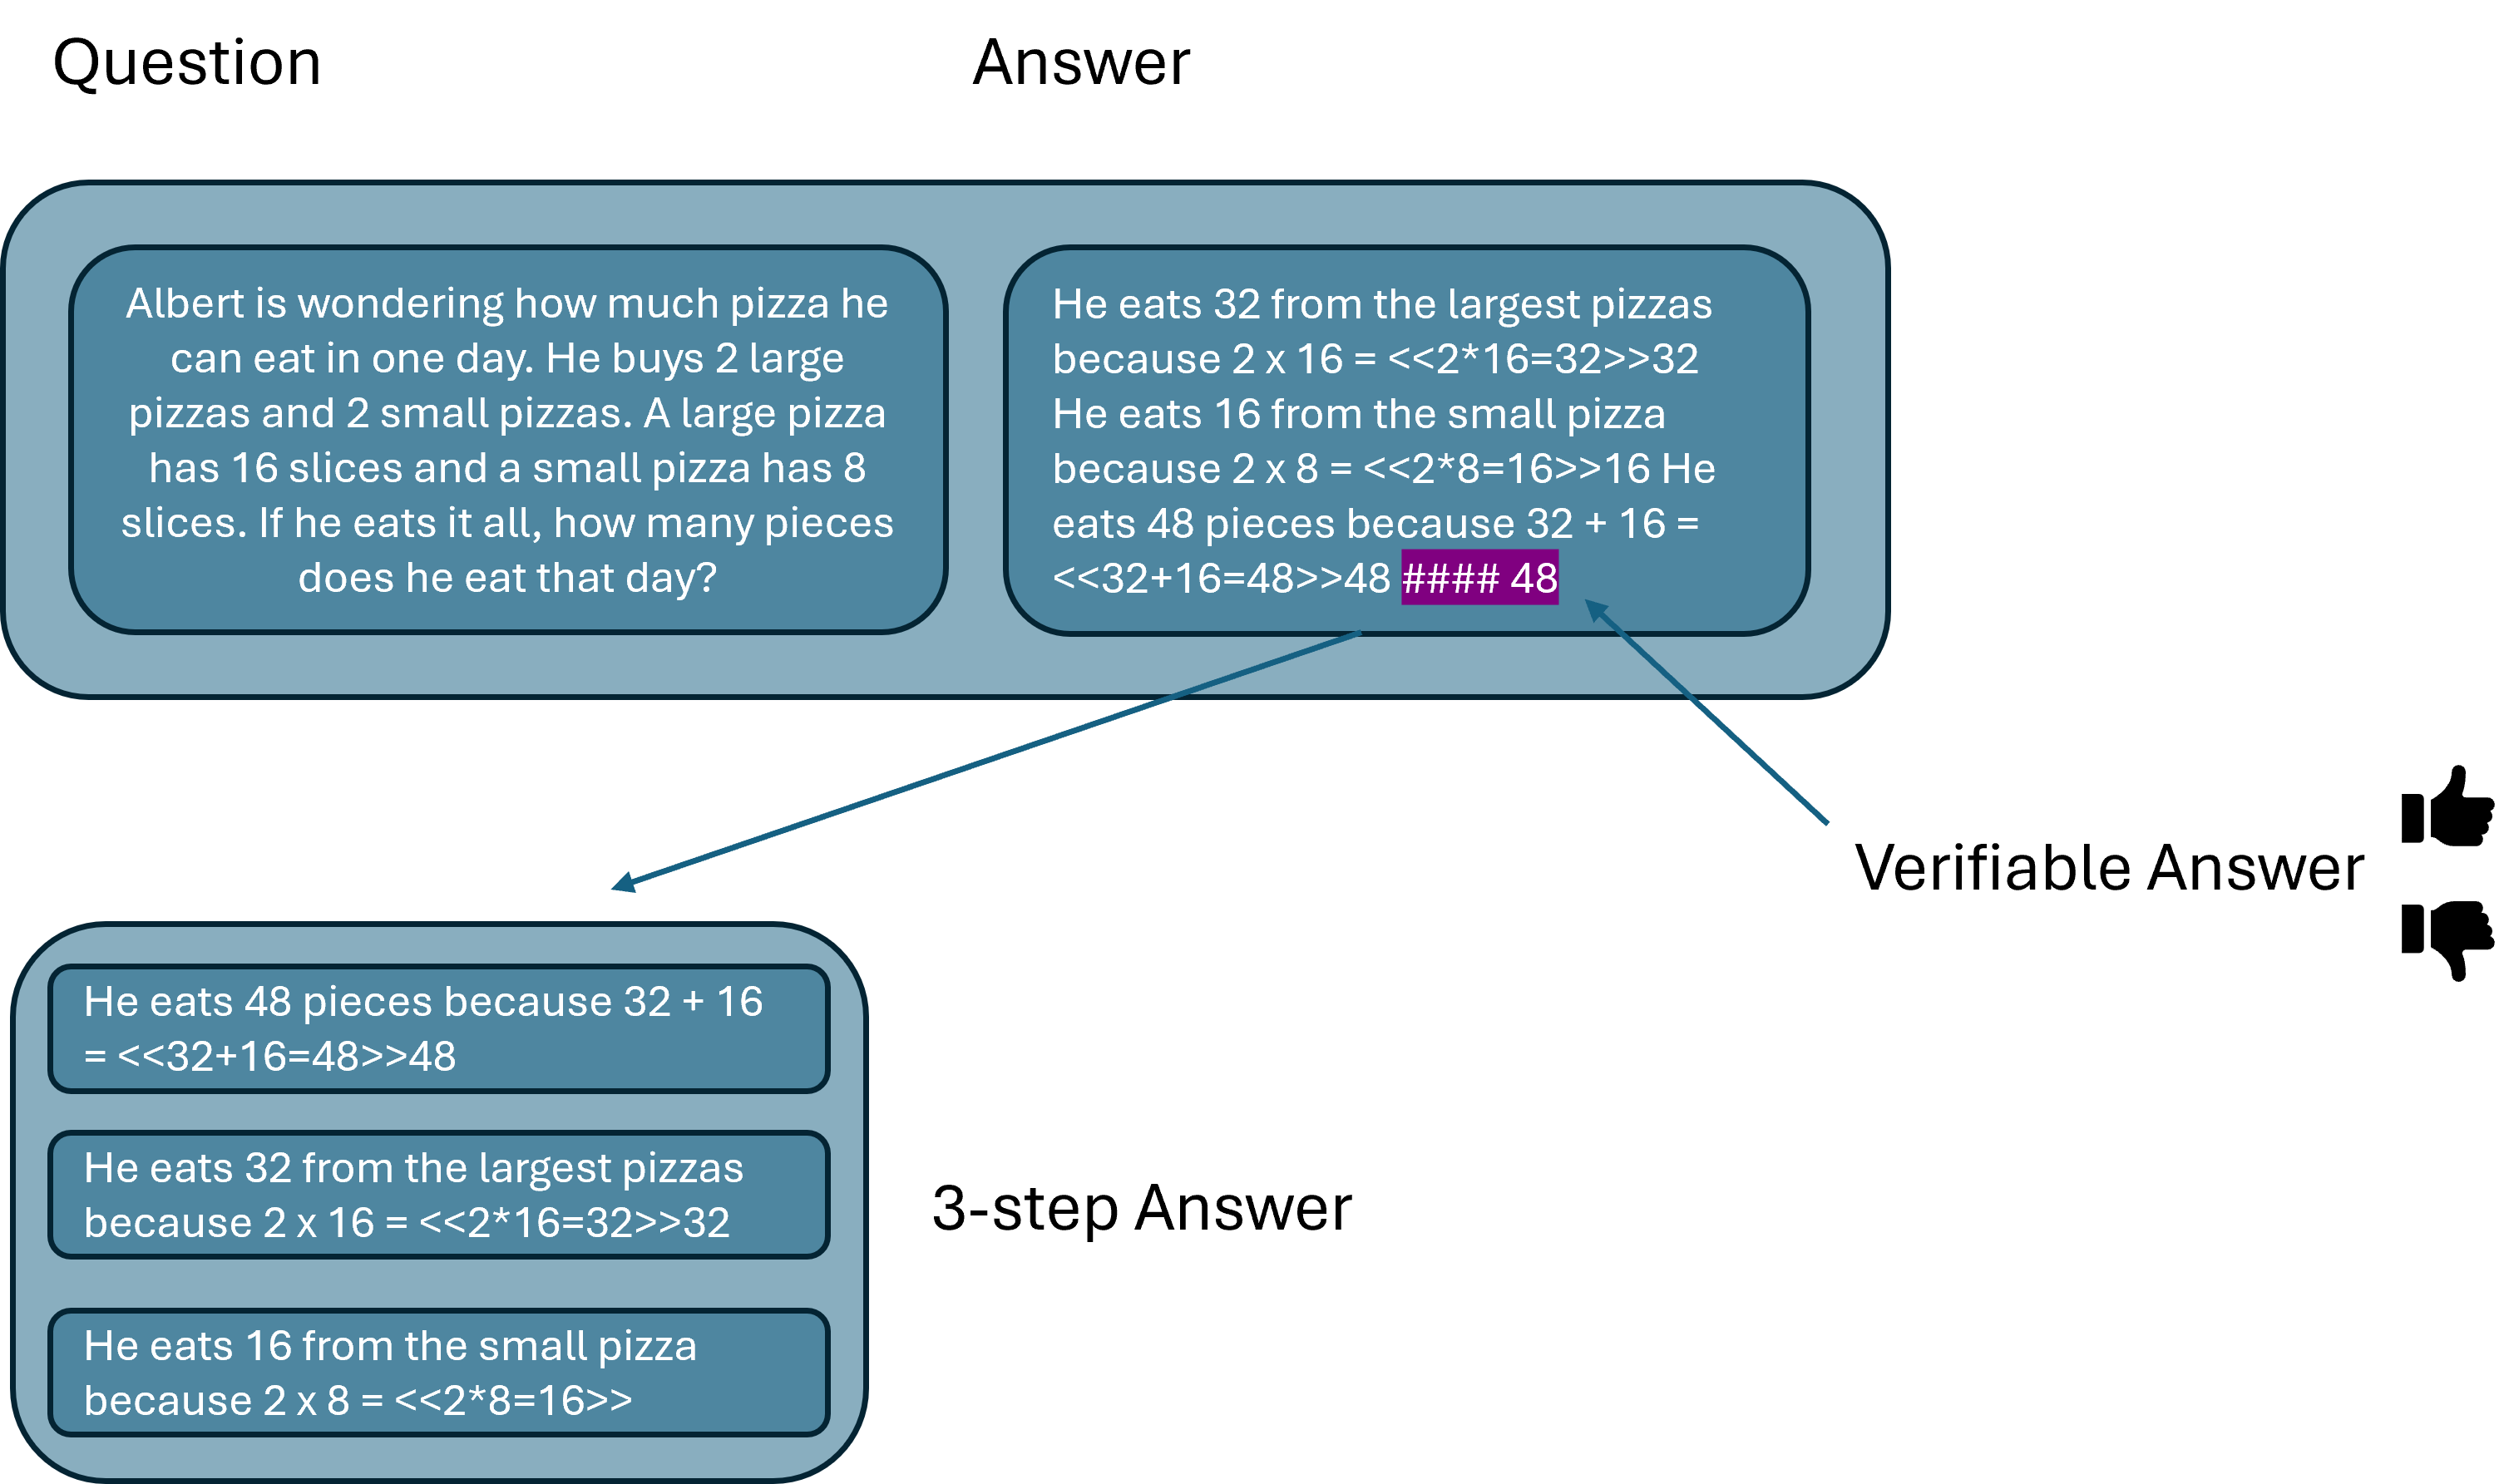
\includegraphics[scale=0.3]{figures/dataset_example}
%\caption{Example of a instance in the GSM8k, for simplicity we removed the special characters in the actual setup}
%\end{figure}

\subsection{Evaluation}
We use a zeroshot with greeding decoding on the test set to evaluate the performance of the models. Firstly the baseline model without any fine-tunning applied and then we repeat the same procedure with the fine-tuned models. In order to compare them we compute the accuracy as  $accuracy = correct \div total$. We use [cite lm-eval] with the flexible extraction mechanism to find the number corresponding to the answer, which simply uses the last occurence of a regex pattern that allow for some non-numeric characters to be included in the answer and will count them as correct. Aditionally we test our method against fine-tunning using the gold labels from the dataset, providing a perspective on improvement on the already available data.





























\end{document}
